% ============================
% REVTeX 4.2e (revtex4-2) + AAPM Template
% ============================
\documentclass[
  aapm,
  amsmath,amssymb,
  reprint,          % journal-like two-column layout
  %preprint,        % uncomment for single-column draft
  floatfix
]{revtex4-2}

% ----------------------------
% Packages
% ----------------------------
\usepackage{graphicx}   % figures
\usepackage{dcolumn}    % decimal-aligned columns in tables
\usepackage{bm}         % bold math
\usepackage{siunitx}    % SI units (optional, nice for reports)
\usepackage{hyperref}   % hyperlinks
\usepackage{placeins}

% Optional: nicer captions (REVTeX already formats captions well)
% \usepackage[labelfont=bf]{caption}

% ----------------------------
% Title block
% ----------------------------
\begin{document}

\title{Project 1: Numerical Solutions to Elliptic PDEs} % <-- change title

\author{Jaden Mecham}
\email{jadenmecham@unr.edu} % optional
\affiliation{Department of Mechanical Engineering, University of Nevada, Reno}

\date{\today}

\begin{abstract}
  This project implements and analyzes numerical solutions to the two-dimensional heat equation
  with a spatially varying source term $\kappa(x,y)$, where the steady-state solution satisfies
  the Poisson equation. The spatial domain is discretized using a uniform grid with second-order
  central finite differences, and the resulting linear system is solved using a conjugate gradient
  (CG) method. Mixed boundary conditions are imposed: Dirichlet conditions on the west and north
  boundaries, and Neumann conditions on the east and south boundaries. The transient heat equation
  is solved using Crank--Nicolson time integration, which is unconditionally stable and
  second-order accurate in time, allowing for larger timesteps than explicit methods. Marching
  from the initial condition $u(x,y,0) = 0$, the transient solution converges to the steady state
  at $t^* = 362.4$ (3624 timesteps at $dt = 0.1$), satisfying the convergence criterion
  $\|u(x,y,t) - \tilde{u}(x,y)\|_2 / \|\tilde{u}(x,y)\|_2 < 10^{-4}$. The steady-state
  solution obtained from the transient simulation closely matches the direct Poisson solution,
  confirming the correctness of both implementations and the expected physical behavior of the
  system.
\end{abstract}

\maketitle

% ============================
% Main text
% ============================

\section{Introduction}

Developed in 1822 by Joseph Fourier, the heat equation aims to model how quanities like heat
diffuse through a space. It is now a fundamental concept in physics, engineering, and 
mathematics. In this project, we implement a numerical solution to the 2D heat equation with 
a spatially varying source term $\kappa(x,y)$, whose steady state solution satisfies the 
Poisson equation.


\section{Governing Equations and Boundary Conditions}

The heat equation of interest for this project is given by:

\begin{equation}
\frac{\partial u}{\partial t} = \alpha\left(\frac{\partial^2 u}{\partial x^2} + \frac{\partial^2 u}{\partial y^2}\right) + \kappa(x,y),
\end{equation}

where $u(x,y,t)$ is the temperature distribution, $\alpha$ is the thermal diffusivity, 
and $\kappa(x,y)$ is the spatially varying source term. The following equation 
defines the source term:

\begin{equation}
  \kappa(x,y) = 0.02\, e^{-(x-0.7)^2/0.09 \;-\; (y-0.6)^2/0.25}
\end{equation}

A heatmap of the source term $\kappa(x,y)$ is shown in Figure~\ref{fig:source}, 
which shows a localized heat source centered around $(0.7, 0.6)$.
The steady-state solution $\bar{u}(x,y)$ satisfies the Poisson equation:

\begin{equation}
\alpha\left(\frac{\partial^2 \bar{u}}{\partial x^2} + \frac{\partial^2 \bar{u}}{\partial y^2}\right) = -\kappa(x,y).
\end{equation}

\begin{figure}[h]
  \centering
  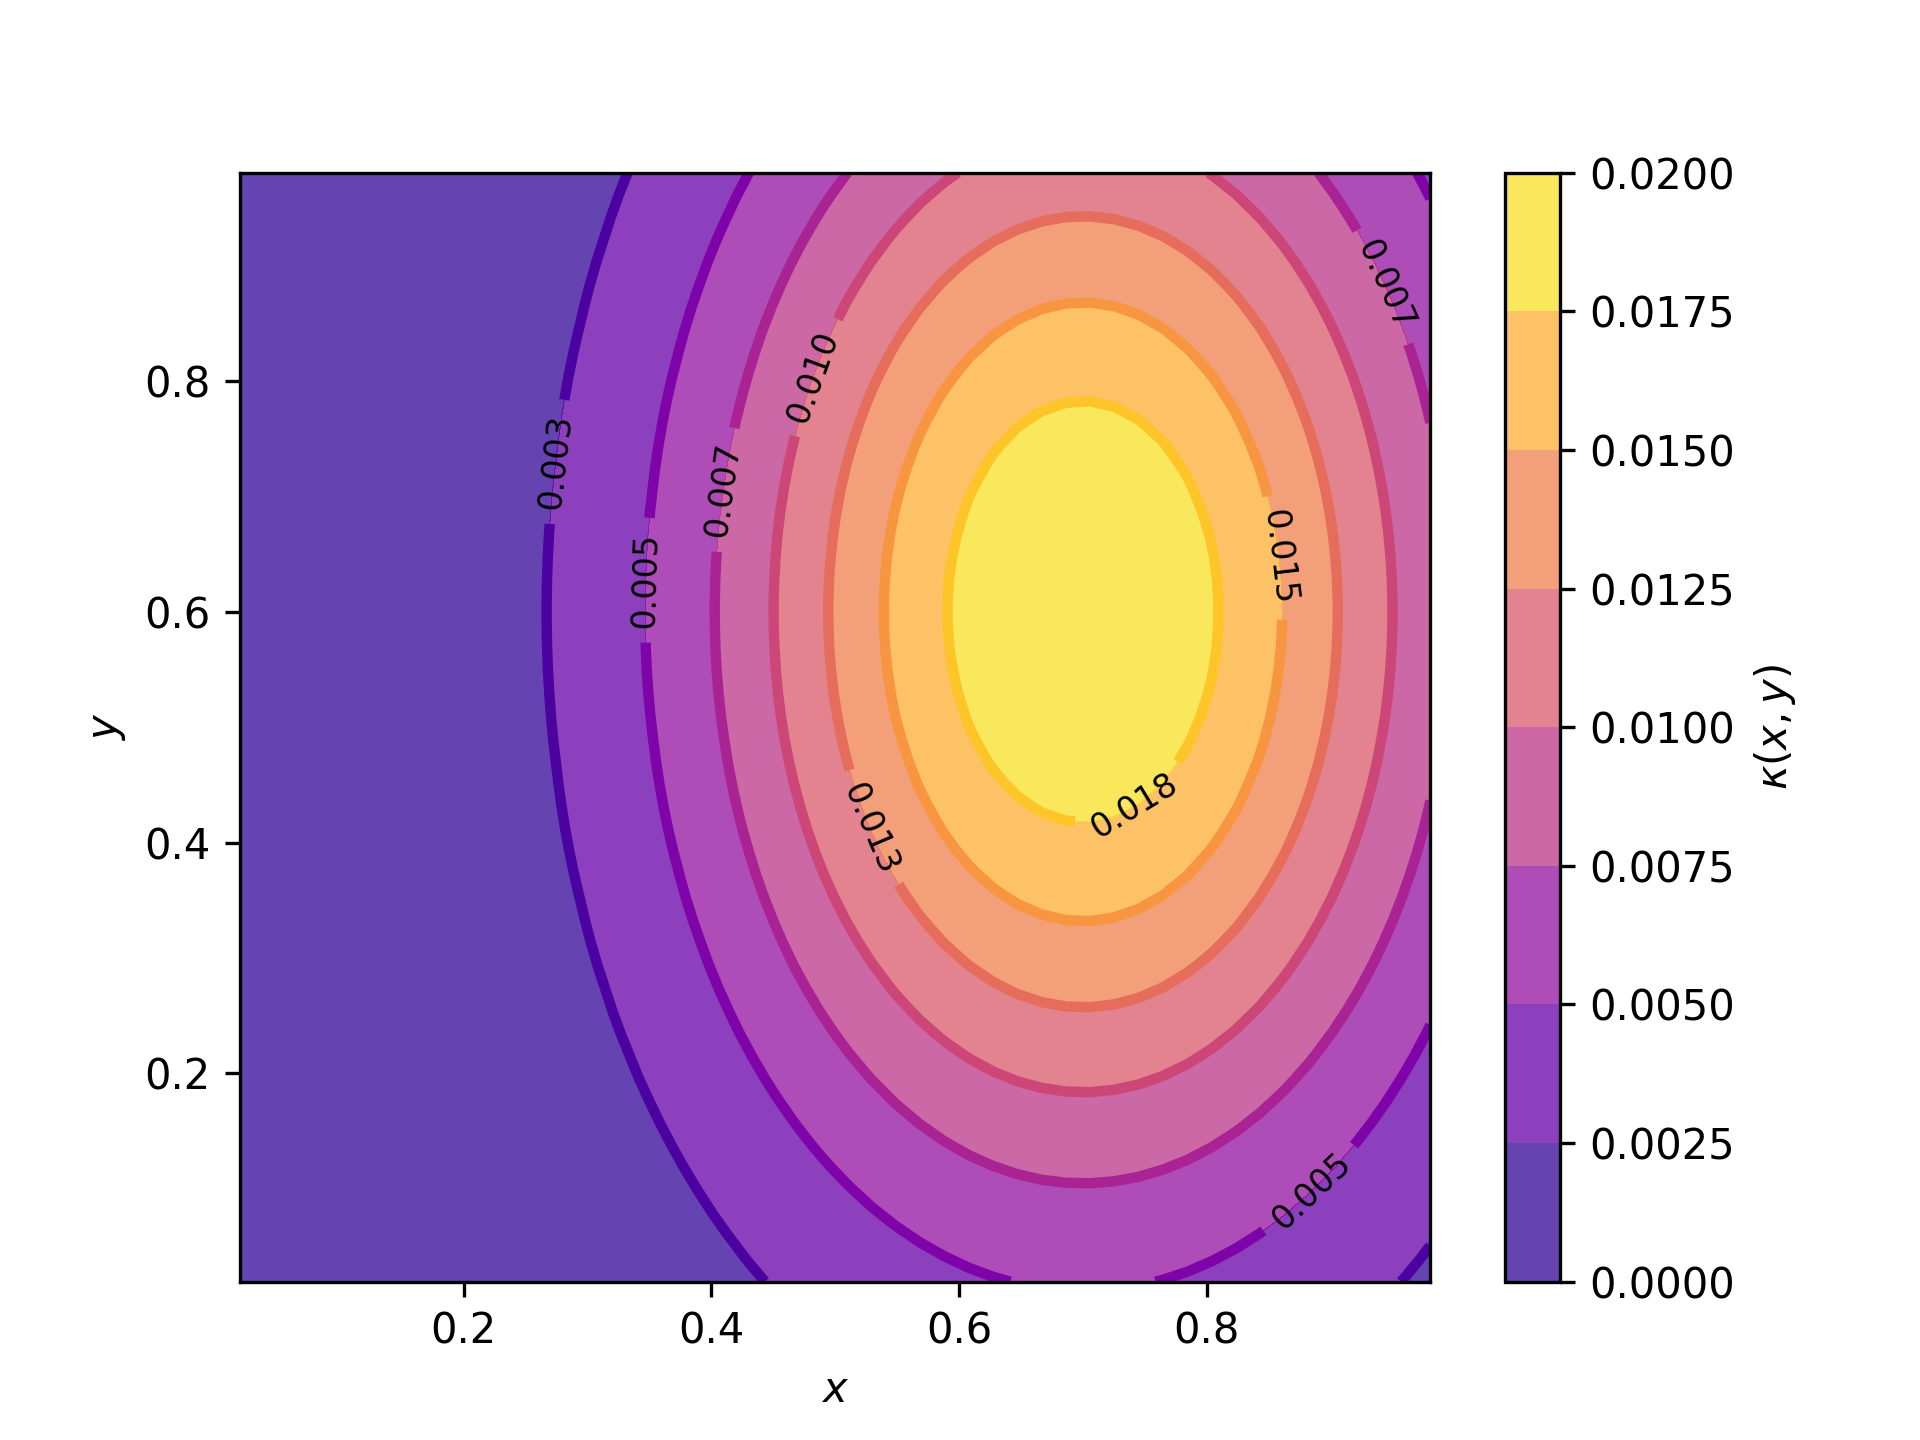
\includegraphics[width=\linewidth]{contour_kappa.png}
  \caption{Contour of source term $\kappa(x,y)$}
  \label{fig:source}
\end{figure}

This problem uses mixed boundary conditions on the domain $[0,1]\times[0,1]$. The west
and north boundaries have Dirichlet conditions while the east and south boundaries have 
Neumann conditions. The boundary conditions are defined in table~\ref{tab:bc}. 
Here, the west boundary condition creates a cosine variation in temperature along the $y$-axis,
while the north boundary condition creates a sine variation along the $x$-axis. The Neumann 
conditions on the east and south boundaries specify a zero flux and a constant negative flux, 
respectively, which influence the overall temperature distribution and the transient behavior 
of the system.

\begin{table}[h]
  \centering
  \caption{Boundary conditions applied to the square domain $[0,1]^2$.}
  \label{tab:bc}
  \begin{tabular}{llll}
  \hline\hline
  Boundary & Location & Type & Condition \\
  \hline
  West  & $x = 0$ & Dirichlet & $u = 0.5 - 0.5\cos(2\pi y)$ \\
  East  & $x = 1$ & Neumann   & $\partial_x u = 0$ \\
  South & $y = 0$ & Neumann   & $\partial_y u = -0.3$ \\
  North & $y = 1$ & Dirichlet & $u = 0.5 + 0.5\sin\!\left(4\pi x - \tfrac{\pi}{2}\right)$ \\
  \hline\hline
  \end{tabular}
  \end{table}

\section{Numerical Method}
\subsection{Grid and Discretization}

The first step in solving this heat equation is defining the spatial grid and discretization.
In this case, the domain $[0,1]\times[0,1]$ is discretized into a uniform grid with 50 elements
in each direction. Therefore, the grid spacing is $h_x = h_y = 1/50$. This divides the domain
into a total of $50\times 50$ grid points, where the temperature $u$ is defined at each point. 

Another important aspect of this process is assigning pointers to the grid points. This gives 
each point a unique index that can be used to reference a specific location instead of needing
to index by $x$ and $y$ coordinates. For example, a $3\times 3$ grid would have the following 
indexing without pointers:
\begin{equation}
\begin{bmatrix}
u(0,2) & u(1,2) & u(2,2) \\
u(0,1) & u(1,1) & u(2,1) \\
u(0,0) & u(1,0) & u(2,0)
\end{bmatrix}
\end{equation}
With pointers, the same grid would be indexed as:

\begin{equation}
\begin{bmatrix}
u_2 & u_5 & u_8 \\
u_1 & u_4 & u_7 \\
u_0 & u_3 & u_6
\end{bmatrix}
\end{equation}

Overall, this makes it easier to reference specific grid points when constructing 
the linear system for the Poisson equation and when implementing the time integration 
for the heat equation.

On the uniform grid, the second-order central finite difference approximation is used to
discretize the spatial derivatives. The 5-point Laplacian stencil for a grid point $(i,j)$ 
is given by:

\begin{equation}
\begin{split}
(\mathbf{L}Q)_{i,j} &= \frac{Q_{i-1,j} - 2Q_{i,j} + Q_{i+1,j}}{\Delta x^2} \\
                    &+ \frac{Q_{i,j-1} - 2Q_{i,j} + Q_{i,j+1}}{\Delta y^2}
\end{split}
\end{equation}

In the interior of the domain, this stencil is applied directly. Near the boundaries, 
This stencil is not directly applied since the boundary conditions must be applied. 
This is done by modifying the stencil to incorporate the boundary conditions, which may involve
using ghost points or directly substituting the boundary values into the equations. For example,
at the west boundary where $u(0,y) = 0.5 - 0.5\cos(2\pi y)$, the stencil for the point adjacent 
to the boundary would be modified to include this Dirichlet condition, 
ensuring that the influence of the boundary is correctly represented in the numerical solution.


\subsection{Linear System and Solver (Poisson)}

The steady-state solution is found by solving the linear system $A\mathbf{u} = \mathbf{b}$, 
where $A$ is the sparse matrix representing the discretized Laplacian operator with boundary 
conditions applied, $\mathbf{u}$ is the vector of unknown temperatures at the grid points, 
and $\mathbf{b}$ is the vector representing the source term $\kappa(x,y)$ and contributions 
from boundary conditions. The conjugate gradient method is used to solve this linear system 
efficiently, especially given the sparsity of $A$. The solver is configured with a 
tolerance of $10^{-6}$ for convergence and a maximum of 1000 iterations. 
The stopping criterion for the solver is based on the relative residual norm, 
ensuring that the solution is sufficiently accurate before termination.

\subsection{Time Integration (Heat Equation)}

The time marching method used to solve the transient heat equation is the Crank--Nicolson method, 
which is an implicit time integration scheme that is second-order accurate in time and 
unconditionally stable. The time step $dt$ is set to 0.1, allowing for larger time 
steps and fewer iterations required. The stopping criterion for the simulation 
is based on the $L^2$ norm of the difference between the transient solution $u(x,y,t)$ 
and the steady-state solution $\bar{u}(x,y)$ from the Poisson solver. 
The simulation is considered to have converged to steady state when:

\begin{equation}
\frac{\|u(x,y,t) - \bar{u}(x,y)\|_2}{\|\bar{u}(x,y)\|_2} < 10^{-4}
\end{equation}

\section{Results}
\subsection{Poisson Steady-State Solution}

Figure \ref{fig:poisson} shows the steady-state solution $\bar{u}(x,y)$ obtained by solving 
the Poisson equation.

\begin{figure}[h]
  \centering
  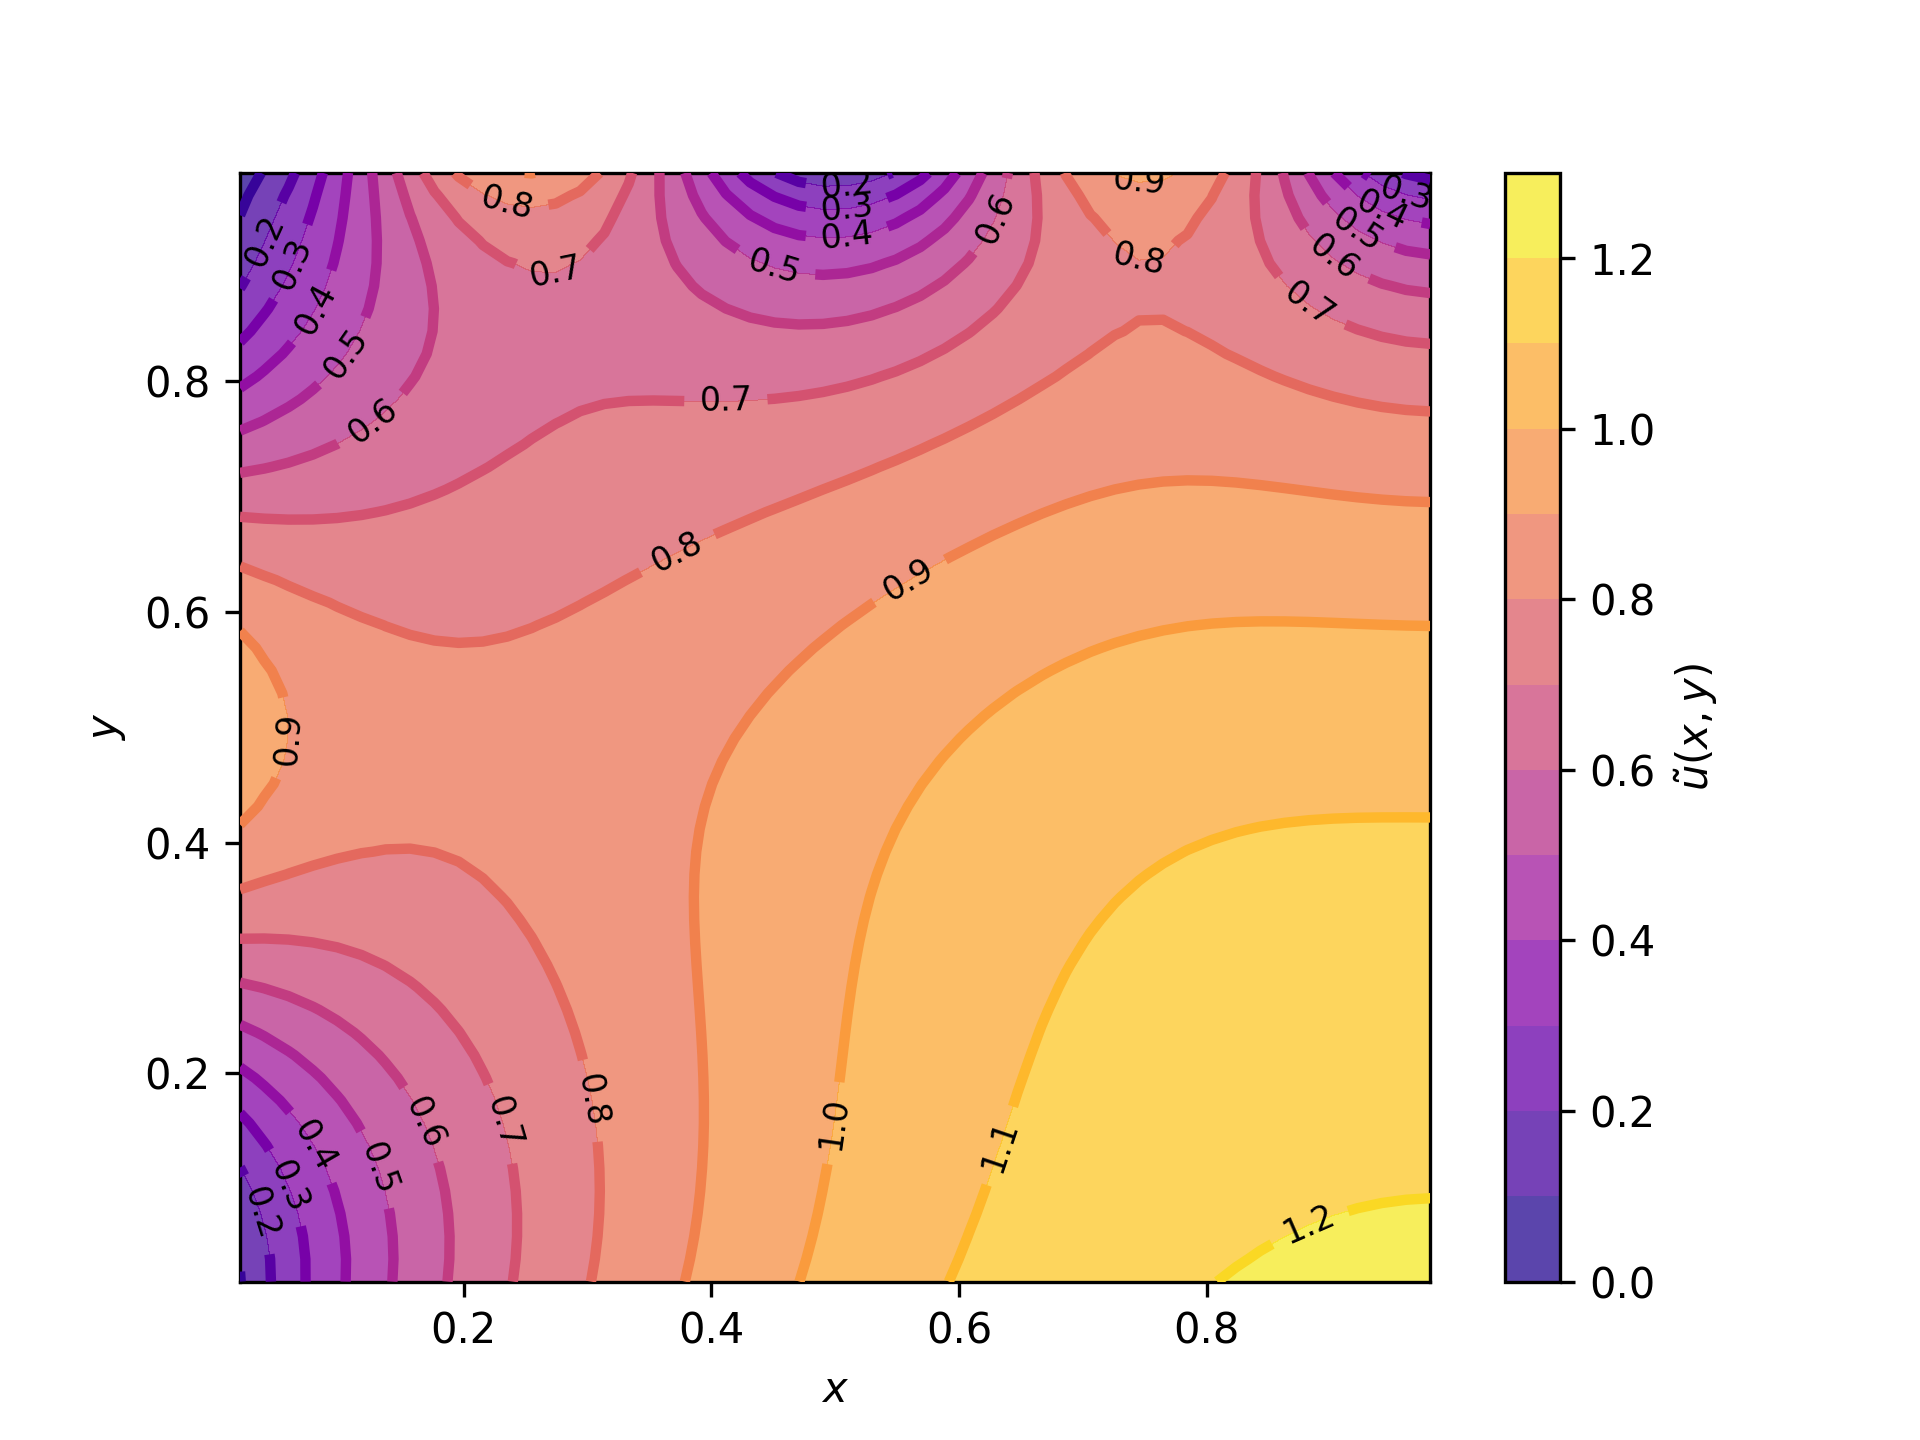
\includegraphics[width=\linewidth]{solution_contour.png}
  \caption{Steady-state solution $\bar{u}(x,y)$ obtained by solving the Poisson equation
  using second-order finite differences and conjugate gradient.}
  \label{fig:poisson}
\end{figure}

Along the North boundary, the solution shows 3 sinks corresponding to the 3 peaks in the 
Dirichlet condition. The solution also shows a peak in the southeast corner, which is influenced 
by the Neumann condition and the source term $\kappa(x,y)$. Furthermore, the southwest corner
shows another sink, which is influenced by the Neumann condition on the south boundary 
and the source term.

\subsection{Transient Heat Equation and Settling Time}

Figure \ref{fig:transient} shows the transient solution $u(x,y,t)$ at selected timesteps as 
it marches from $u(x,y,0) = 0$ to the steady state. The solution evolves over time, 
with the temperature distribution gradually changing as it approaches the steady-state solution. 
The transient solution converges to the steady state at $t^* = 362.4$ 
(3624 timesteps at $dt = 0.1$), satisfying the convergence criterion based on the $L^2$ norm 
of the difference between the transient and steady-state solutions.

\begin{figure*}
  \centering
  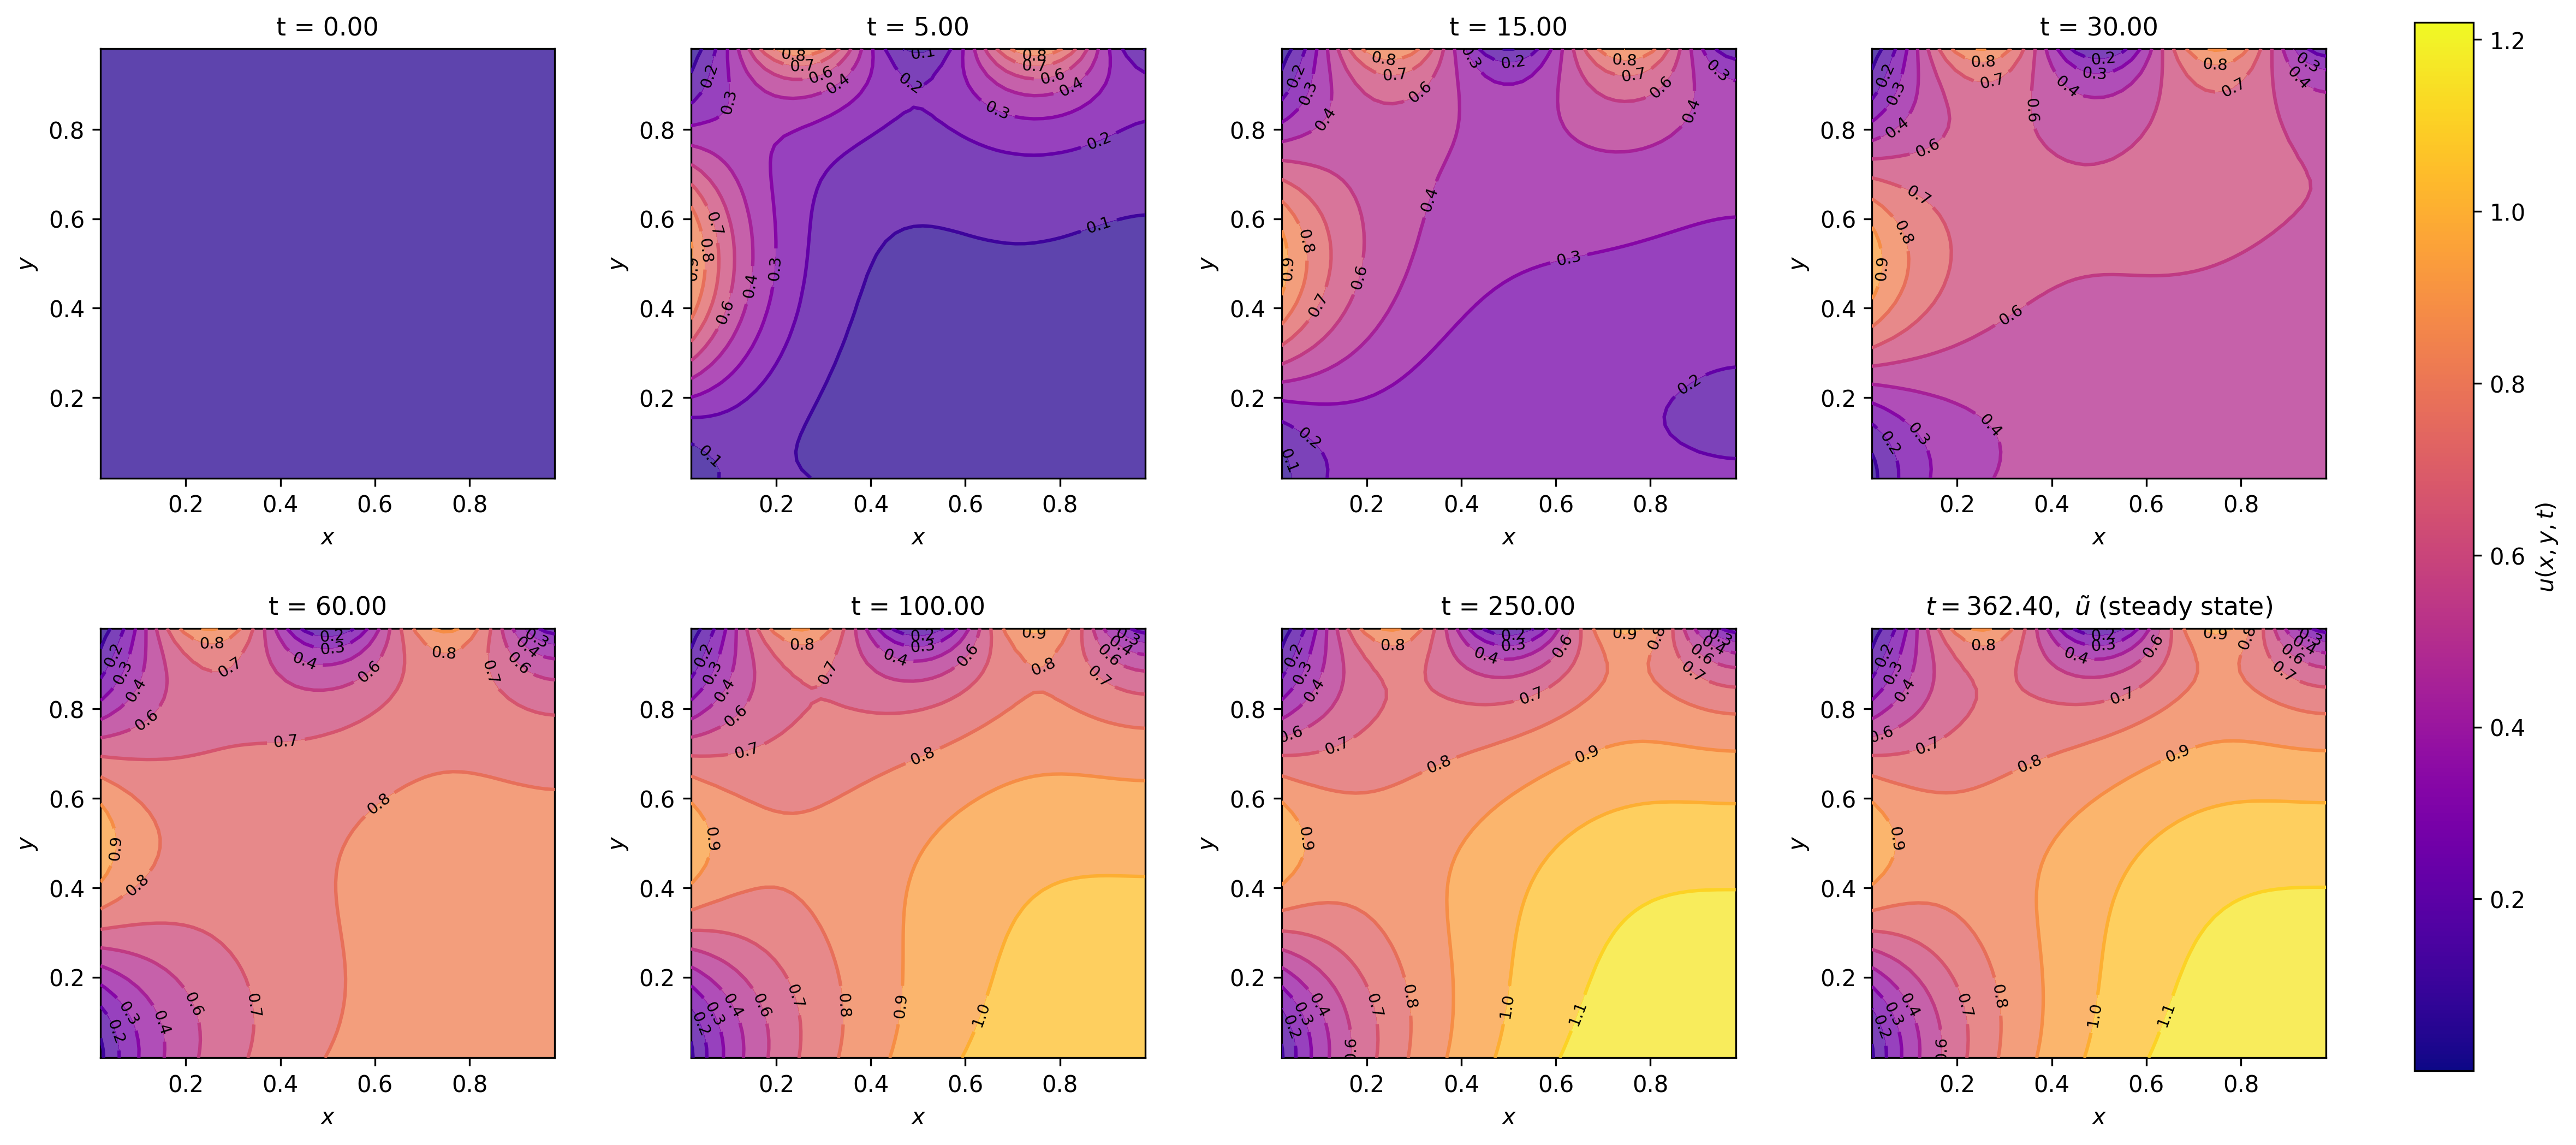
\includegraphics[width=\linewidth]{solution_timesteps.png}
  \caption{Transient solution $u(x,y,t)$ at selected timesteps, marching from
  $u(x,y,0)=0$ to steady state using Crank--Nicolson time integration.}
  \label{fig:transient}
\end{figure*}


\subsection{Grid Sensitivity (Optional but Recommended)}
Briefly show that results are mesh-independent (e.g., $21\times 21$, $31\times 31$).

\section{Discussion}
Interpret results: solver performance, convergence trends, stability constraints (if explicit),
and any numerical issues (boundary treatment, corners, conditioning, etc.).

\section{Conclusion}
Summarize the main takeaways in 4--6 sentences. Clearly state the final reported settling time
and the steady-state match.

% ============================
% References
% ============================
\bibliographystyle{aapmrev4-2}
% Option A: BibTeX file (recommended)
\bibliography{references}

% Option B: Manual references (if you don't want BibTeX)
% \begin{thebibliography}{99}
% \bibitem{smith2020} J. Smith, \textit{Numerical PDEs} (Publisher, 2020).
% \end{thebibliography}

\end{document}
